\documentclass[a4paper]{article}
\usepackage[utf8]{inputenc}
\usepackage[russian,english]{babel}
\usepackage[T2A]{fontenc}
\usepackage[left=10mm, top=20mm, right=18mm, bottom=15mm, footskip=10mm]{geometry}
\usepackage{indentfirst}
\usepackage{amsmath,amssymb}
\usepackage[italicdiff]{physics}
\usepackage{graphicx}
\usepackage{multirow}
\usepackage{svg}
\graphicspath{{images/}}
\DeclareGraphicsExtensions{.pdf,.png,.jpg}
\usepackage{wrapfig}
\usepackage{caption}
\captionsetup[figure]{name=Рисунок}
\captionsetup[table]{name=Таблица}
\title{\underline{Магнитометр}}
\author{Каспаров Николай, Б01-304}

\begin{document}

\maketitle
\begin{center}
\Large{\textbf{ }}
\end{center}

\subparagraph{Цель работы:}

\begin{itemize}
\item Определить горизонтальную составляющую магнитного поля Земли;
\item Установить количественное соотношение между единицами электрического тока в системах СИ и СГС.
\end{itemize}

\subparagraph{В работе используются:}

В работе используются: магнитометр, осветитель со шкалой, источник питания,
вольтметр, электромагнитный переключатель, конденсатор, намагниченный стержень,
прибор для определения периода крутильных колебаний,
секундомер, рулетка, штангенциркуль.

\section{Экспериментальная установка}

\begin{figure}[h!]
    \centering
    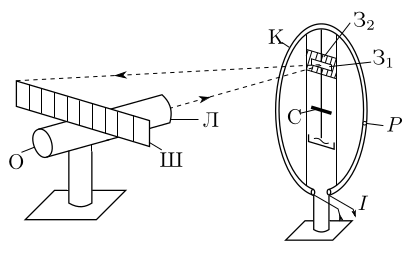
\includegraphics[width=0.5\pdfpagewidth]{shema.png}
    \caption{Схема магнитометра}
\end{figure}
Магнитометр (рис. 1) состоит из нескольких последовательно соединённых круговых витков К,
расположенных вертикально.
В центре кольца К радиусом R на тонкой неупругой вертикальной нити подвешена короткая магнитная стрелка С.

В отсутствие других магнитных полей стрелка располагается по направлению
горизонтальной составляющей земного магнитного поля $B_0$.
\begin{figure}[h!]
    \centering
    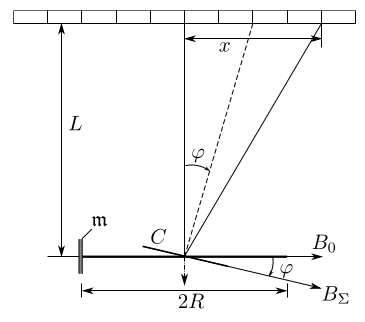
\includegraphics[width=0.4\pdfpagewidth]{2.png}
    \caption{Схема измерения угла отклонения магнитной стрелки}
\end{figure}

Прибор настраивают с помощью световых зайчиков, отражённых от двух зеркал: $\text{З}_1$,
прикреплённого к стрелке (подвижный зайчик), и $\text{З}_2$,
расположенного в плоскости кольца К и жёстко связанного с ним (неподвижный зайчик).
Оба зеркала освещаются одним и тем же осветителем О.
Вращением кольца вокруг вертикальной оси можно совместить оба зайчика.
При этом плоскость витков совпадает с плоскостью магнитного меридиана.

При появлении дополнительного горизонтального магнитного поля $B_\perp$,
стрелка C установится по равнодействующей обоих полей $B_\Sigma$ (рис. 2).
В нашей установке дополнительное поле может быть создано либо малым ферромагнитным стержнем,
расположенным на кольце на его горизонтальном диаметре ($B_1$), либо током, проходящим по кольцу ($B_2$).
В обоих случаях дополнительное поле можно считать однородным, так как размеры стрелки много меньше радиуса кольца.

Поле намагниченного стержня вдали от него может быть приближённо вычислено как поле точечного диполя:

\begin{equation*}
    \vec{B}(r) = \frac{\mu_0}{4\pi} \left( 3\frac{(\vec{m} \cdot \vec{r}) ~\vec{r} }{r^5} - \frac{\vec{m}}{r^3}\right),
\end{equation*}
где $\vec{m}$ - магнитный момент стержня, 

\noindent $\vec{r}$ - радиус-вектор, проведённый из центра диполя в точку наблюдения.

На оси, перпендикулярной стержню, имеем:

\begin{equation}
    B_1 = \frac{\mu_0}{4\pi} \frac{m}{R^3},
\end{equation}
где $R$ - радиус кольца.

Магнитное поле в центре кольца с током $I$ по закону Био — Савара — Лапласа равно:

\begin{equation}
    B_2 = \frac{\mu_0I}{2R}N,
\end{equation}
где $N$ - число витков в кольце, $I$ [A] - сила тока.

Измерив угол отклонения стрелки $\varphi$, можно связать поля $B_0$ и $B_\perp$
($B_1$ или $B_2$):
\begin{equation}
    B_\perp = B_0 \cdot \tg{\varphi}
\end{equation}

\subsection{Определение горизонтальной составляющей магнитного поля Земли}

Для определения горизонтальной составляющей земного магнитного
поля $B_0$ тонкий короткий намагниченный стержень устанавливается в
отверстие $Р$ на горизонтальном диаметре кольца (рис. 1).
Измерив тангенс угла отклонения стрелки

\begin{equation}
    \tg{\varphi_1} = \frac{x_1}{2L},
\end{equation}
можно с помощью уравнений (1), (3) и (4) рассчитать поле $B_0$,
если исключить величину m — магнитный момент стержня.

Для исключения магнитного момента предлагается измерить период крутильных колебаний стержня в поле Земли.
Подвешенный горизонтально за середину на тонкой длинной нити стержень в положении
равновесия установится по полю Земли.
Если ось стержня отклонить в горизонтальной плоскости от
направления $B_0$ на малый угол $\alpha$,
то под действием возвращающего механического момента
\begin{equation*}
    M_\text{мех} = |\vec{m} \crossproduct \vec{B}| = mB_0 \sin{\alpha} \approx mB_0\alpha
\end{equation*}
стержень с моментом инерции $J$ в соответствии с уравнением
\begin{equation*}
    J \ddot{\alpha} + mB_0\alpha = 0
\end{equation*}
будет совершать крутильные колебания c периодом
\begin{equation}
    T = 2\pi \sqrt{\frac{J}{mB_0}}.
\end{equation}

Момент инерции цилиндрического стержня относительно оси вращения
\begin{equation}
    J = m \left( \frac{l^2}{12} + \frac{r^2}{4} \right) = \frac{ml^2}{12} \left[ 1 + 3\left(\frac{r}{l}\right)^2\right]
\end{equation}

Таким образом, из (1), (3), (4) и (5) следует:
\begin{equation}
    B_0 = \frac{2\pi}{RT}\sqrt{\frac{\mu_0JL}{2\pi Rx_1}} \qquad \text{[ед. СИ]}
\end{equation}

\subsection{Определение электродинамической постоянной}

Пропуская некоторый ток через витки магнитометра, измерим тангенс угла отклонения стрелки\\
$(\tg{\varphi_2} = x_2 /2L)$ и по формулам (2) и (3) рассчитаем силу тока:

\begin{equation}
    I = \frac{2B_0 R}{\mu_0 N} \tg{\varphi_2} = A \tg{\varphi_2} \qquad \text{[ед. СИ]},
\end{equation}
где $A$ - постоянная прибора и места.

Тот же ток можно измерить абсолютным образом по прошедшему в единицу времени заряду,
что соответствует определению эталона тока в гауссовой системе (СГС).
Если разрядить конденсатор известной ёмкости $C$, заряженный до напряжения $U$,
через витки, то через них протечёт заряд $q$ = $CU$ (рис. 3). Если $\nu$ раз в секунду последовательно
заряжать конденсатор от источника и разряжать через витки, то через
них за секунду протечёт заряд $CU\nu$.
Средний ток, прошедший через витки, равен при этом
\begin{equation}
    I = CU\nu \qquad \text{[абс. ед]}
\end{equation}

\begin{figure}[h!]
    \centering
    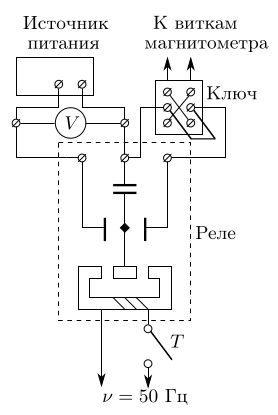
\includegraphics[width=0.3\pdfpagewidth]{3.png}
    \caption{Схема питания катушки магнитометра}
\end{figure}

Таким образом, абсолютное измерение тока сводится к нахождению величин $C$ и $U$,
которые тоже могут быть определены абсолютным образом.
По отношению численных значений одного и того же тока, выраженных в единицах СИ и СГС,
можно определить значение электродинамической постоянной:
\begin{equation}
    c = \frac{1}{10} \frac{I_\text{СГС}}{I_\text{СИ}} \ \text{[м/с]}
\end{equation}

\section{Ход работы}

\subsection{Измерение горизонтальной составляющей магнитного поля Земли}

Намагниченный стержень вызвал отклонение зайчика $x_1 = (95 \pm 1)~\text{мм}$, $x_2 = (-94 \pm 1)~\text{мм}$

\noindent Параметры установки:
\begin{equation*}
    L = (0.84 \pm 0.05)~\text{м}
\end{equation*}
\begin{equation*}
    R = (0.25 \pm 0.01)~\text{м}
\end{equation*}

\noindent Параметры намагниченного стержня:
\begin{equation*}
    m = (2.84 \pm 0.01)~\text{гр}
\end{equation*}
\begin{equation*}
    l = (24.3 \pm 0.1)~\text{мм}
\end{equation*}
\begin{equation*}
    d = (4.6 \pm 0.1)~\text{мм}
\end{equation*}

\noindent Посчитаем момент инерции магнита по формуле (6):
\begin{equation*}
    J = \frac{ml^2}{12} \left[ 1 + 3\left(\frac{r}{l}\right)^2\right] = (1.44 \pm 0.04) \cdot 10^{-7}~\text{кг}\cdot\text{м}^2
\end{equation*}

\noindent Определим период колебания магнита в горизонтальной плоскости:
\begin{equation*}
    T = (1.79 \pm 0.09) ~c
\end{equation*}

\noindent Горизонтальное магнитное поле Земли по формуле (7);
\begin{equation*}
    B_0 = \frac{2\pi}{RT}\sqrt{\frac{\mu_0JL}{2\pi R\overline{x}}} = (1.4 \pm 0.2)\cdot 10^{-5}
\end{equation*}

\subsection{Определение электродинамической постоянной}
\noindent Параметры установки:
\begin{equation*}
    N = 34
\end{equation*}
\begin{equation*}
    \nu = 50 ~\text{Гц}
\end{equation*}
\begin{equation*}
    U = (0.336 \pm 0.001) ~\text{ед. СГС}
\end{equation*}
\begin{equation*}
    C = (9.0 \pm 0.1) \cdot 10^5 ~\text{см}
\end{equation*}

\noindent Смещение зайчика: 
\begin{equation*}
    x_1 = (7.5 \pm 0.1) ~\text{см}
\end{equation*}
\begin{equation*}
    x_2 = (-8.0 \pm 0.1) ~\text{см}
\end{equation*}

\noindent Сила тока в системе СИ, формула (8):
\begin{equation*}
    I = \frac{2B_0 R}{\mu_0 N} \tg{\varphi_2} = (5.2 \pm 0.8) \cdot 10^{-3} ~\text{[А]},
\end{equation*}

\noindent Сила тока в системе СГС, формула (9):
\begin{equation*}
    I = CU\nu = (1.51 \pm 1) \cdot 10^7 ~\text{ед. СГС}.
\end{equation*}

\noindent Отсюда, значение электродинамической постоянной равно:

\begin{equation*}
    c = \frac{1}{10} \frac{I_\text{СГС}}{I_\text{СИ}} = (2.9 \pm 0.4) \cdot 10^8 \ \text{м/с}
\end{equation*}

\section{Вывод}

Во время выполнения данной работы, удалось рассчить величину горизонтальной составляющей магнитного поля Земли.
\begin{equation*}
    B_0 = (1.4 \pm 0.2)\cdot 10^{-5}
\end{equation*}
А также вычислить электродинамическую постоянную $c$:
\begin{equation*}
    c = (2.9 \pm 0.4) \cdot 10^8 \ \text{м/с}
\end{equation*}

Наименее точным измерением оказалось определение периода магнита.

\end{document}

